% This is "sig-alternate.tex" V2.0 May 2012
% This file should be compiled with V2.5 of "sig-alternate.cls" May 2012
%
% This example file demonstrates the use of the 'sig-alternate.cls'
% V2.5 LaTeX2e document class file. It is for those submitting
% articles to ACM Conference Proceedings WHO DO NOT WISH TO
% STRICTLY ADHERE TO THE SIGS (PUBS-BOARD-ENDORSED) STYLE.
% The 'sig-alternate.cls' file will produce a similar-looking,
% albeit, 'tighter' paper resulting in, invariably, fewer pages.
%
% ----------------------------------------------------------------------------------------------------------------
% This .tex file (and associated .cls V2.5) produces:
%       1) The Permission Statement
%       2) The Conference (location) Info information
%       3) The Copyright Line with ACM data
%       4) NO page numbers
%
% as against the acm_proc_article-sp.cls file which
% DOES NOT produce 1) thru' 3) above.
%
% Using 'sig-alternate.cls' you have control, however, from within
% the source .tex file, over both the CopyrightYear
% (defaulted to 200X) and the ACM Copyright Data
% (defaulted to X-XXXXX-XX-X/XX/XX).
% e.g.
% \CopyrightYear{2007} will cause 2007 to appear in the copyright line.
% \crdata{0-12345-67-8/90/12} will cause 0-12345-67-8/90/12 to appear in the copyright line.
%
% ---------------------------------------------------------------------------------------------------------------
% This .tex source is an example which *does* use
% the .bib file (from which the .bbl file % is produced).
% REMEMBER HOWEVER: After having produced the .bbl file,
% and prior to final submission, you *NEED* to 'insert'
% your .bbl file into your source .tex file so as to provide
% ONE 'self-contained' source file.
%
% ================= IF YOU HAVE QUESTIONS =======================
% Questions regarding the SIGS styles, SIGS policies and
% procedures, Conferences etc. should be sent to
% Adrienne Griscti (griscti@acm.org)
%
% Technical questions _only_ to
% Gerald Murray (murray@hq.acm.org)
% ===============================================================
%
% For tracking purposes - this is V2.0 - May 2012

\documentclass{sig-alternate}

\begin{document}
%
% --- Author Metadata here ---
\conferenceinfo{SIGIR}{'15, August 9-13, 2015, Santiago, Chile}
%\CopyrightYear{2007} % Allows default copyright year (20XX) to be over-ridden - IF NEED BE.
%\crdata{0-12345-67-8/90/01}  % Allows default copyright data (0-89791-88-6/97/05) to be over-ridden - IF NEED BE.
% --- End of Author Metadata ---

\title{Patent Prior-art search Failure  Analysis
%\titlenote{(Produces the permission block, and
%copyright information). For use with
%SIG-ALTERNATE.CLS. Supported by ACM.}
}
\subtitle{Why Patent Prior-art Search Fails?
%\titlenote{A full version of this paper is available as
%\textit{Author's Guide to Preparing ACM SIG Proceedings Using
%\LaTeX$2_\epsilon$\ and BibTeX} at
%\texttt{www.acm.org/eaddress.htm}}
}
%
% You need the command \numberofauthors to handle the 'placement
% and alignment' of the authors beneath the title.
%
% For aesthetic reasons, we recommend 'three authors at a time'
% i.e. three 'name/affiliation blocks' be placed beneath the title.
%
% NOTE: You are NOT restricted in how many 'rows' of
% "name/affiliations" may appear. We just ask that you restrict
% the number of 'columns' to three.
%
% Because of the available 'opening page real-estate'
% we ask you to refrain from putting more than six authors
% (two rows with three columns) beneath the article title.
% More than six makes the first-page appear very cluttered indeed.
%
% Use the \alignauthor commands to handle the names
% and affiliations for an 'aesthetic maximum' of six authors.
% Add names, affiliations, addresses for
% the seventh etc. author(s) as the argument for the
% \additionalauthors command.
% These 'additional authors' will be output/set for you
% without further effort on your part as the last section in
% the body of your article BEFORE References or any Appendices.

\numberofauthors{3} %  in this sample file, there are a *total*
% of EIGHT authors. SIX appear on the 'first-page' (for formatting
% reasons) and the remaining two appear in the \additionalauthors section.
%
\author{
% You can go ahead and credit any number of authors here,
% e.g. one 'row of three' or two rows (consisting of one row of three
% and a second row of one, two or three).
%
% The command \alignauthor (no curly braces needed) should
% precede each author name, affiliation/snail-mail address and
% e-mail address. Additionally, tag each line of
% affiliation/address with \affaddr, and tag the
% e-mail address with \email.
%
% 1st. author
\alignauthor
Sean Fogarty\\%\titlenote{Dr.~Trovato insisted his name be first.}\\
       \affaddr{NICTA \& ANU}\\
       \affaddr{Canberra, Australia}\\
       %\affaddr{Wallamaloo, New Zealand}\\
       \email{\scriptsize name.surname@nicta.com.au}
% 2nd. author
\alignauthor
G.K.M. Tobin\\%\titlenote{The secretary disavows
%any knowledge of this author's actions.}\\
       \affaddr{NICTA \& ANU}\\
       \affaddr{Canberra, Australia}\\
       %\affaddr{Dublin, Ohio 43017-6221}\\
       \email{\scriptsize name.surname@nicta.com.au}
% 3rd. author
\alignauthor Lars Th{\o}rv{\"a}ld\\%\titlenote{This author is the
%one who did all the really hard work.}\\
       \affaddr{NICTA \& ANU}\\
       \affaddr{Canberra, Australia}\\
      % \affaddr{Hekla, Iceland}\\
       \email{\scriptsize name.surname@nicta.com.au}
%\and  % use '\and' if you need 'another row' of author names
% 4th. author
%\alignauthor Lawrence P. Leipuner\\
%       \affaddr{Brookhaven Laboratories}\\
%       \affaddr{Brookhaven National Lab}\\
%       \affaddr{P.O. Box 5000}\\
%       \email{lleipuner@researchlabs.org}
% 5th. author
%\alignauthor Sean Fogarty\\
%       \affaddr{NASA Ames Research Center}\\
%       \affaddr{Moffett Field}\\
%       \affaddr{California 94035}\\
%       \email{fogartys@amesres.org}
%% 6th. author
%\alignauthor Charles Palmer\\
%       \affaddr{Palmer Research Laboratories}\\
%       \affaddr{8600 Datapoint Drive}\\
%       \affaddr{San Antonio, Texas 78229}\\
%       \email{cpalmer@prl.com}
}
% There's nothing stopping you putting the seventh, eighth, etc.
% author on the opening page (as the 'third row') but we ask,
% for aesthetic reasons that you place these 'additional authors'
% in the \additional authors block, viz.
%\additionalauthors{Additional authors: John Smith (The Th{\o}rv{\"a}ld Group,
%email: {\texttt{jsmith@affiliation.org}}) and Julius P.~Kumquat
%(The Kumquat Consortium, email: {\texttt{jpkumquat@consortium.net}}).}
\date{30 July 1999}
% Just remember to make sure that the TOTAL number of authors
% is the number that will appear on the first page PLUS the
% number that will appear in the \additionalauthors section.

\maketitle
\begin{abstract}

\end{abstract}

% A category with the (minimum) three required fields
\category{H.3.3}{Information Search and Retrieval}{Query Formulation}
%A category including the fourth, optional field follows...
%\category{D.2.8}{Software Engineering}{Metrics}[complexity measures, performance measures]

\terms{Theory}

\keywords{patent search, Query Reformulation, Data Analysis}

\section{Introduction}
In this work, we looked into patent prior-art problem from data analysis perspective.
\section{Experimental Set ups}

\section{Term Analysis}
The main complain about patent search is insufficient match between the content of patent queries and relevant
patents\cite{magdy2012toward, mahdabi2013leveraging}. However, our analyses showed that only \%20 overlap is sufficient for the system to retrieve a relevant or non-relevant patent at top-100 and except for few queries, non-retrieved relevant patents had enough matched term with the query. So, we start our experiments with term analysis for patent query and retrieved documents. 

\subsection{Discriminative Words}
For our initial experiments, we identified the {\em discriminative words} by positive scoring the words in relevant documents and negative scoring the irrelevant one. 
\begin{equation}
score(t,Q)=Rel(t)-Irr(t) 
 \label{eq:score}
\end{equation}
\begin{displaymath}t\in \lbrace \mbox{terms in top-100 retrieved documents}\rbrace\end{displaymath}
Where $ Rel(t) $ is the average term frequency in retrieved relevant patents and $ Irr(t) $ is the average term frequency in retrieved irrelevant patents. Words with a positive score consider {\em useful words} since they are more frequent in relevant patents while the words with negative score are {\em noisy words} as they appeared more frequently in irrelevant patents. 

Surprisingly, we could not find any correlation between the percentage of {\em useful words} and the performance. We expected a higher performance for the queries with more {\em useful words}. 

\subsubsection{Optimal RF\protect\footnote{Relevance Feedback} Query Formulation}
We hypothesize that a query formulated by {\em useful terms} is optimal since they are all frequent in relevant patents and rare in irrelevant ones. Table \ref{tab:optquery} compares the performance for baseline where the query is the full patent query both weighted and unweighed with the performance for optimal RF query weighted with the score of each term(formula \ref{eq:score}) and unweighed. 

\begin{table}[htpb]
  \begin{center}
   \caption{.}
  \input table/optquery.tex   
  \label{tab:optquery}
  \end{center}  
\end{table}

It can be seen that `MAP' jumps from 0.1618 to \textbf{0.5075} which is about \%35 increase. We use a score threshold($\tau$) to formulate the RF query(we select the terms with $ score(t)>\tau $). Fig. (1-a) indicates two important facts. First, it shows that increasing the threshold results in the lower performance. Second, the system is over-sensitive to the {\em noisy words}($ \tau<0 $).  Fig. (1-b) shows that formulating a query with up to 200 {\em useful words} helps performance whereas the performance improves slightly by adding more than 200 words. 
%Fig. 1 indicates how the score threshold and the query size control the performance. 

%\begin{figure}[htpb]
%\centering
%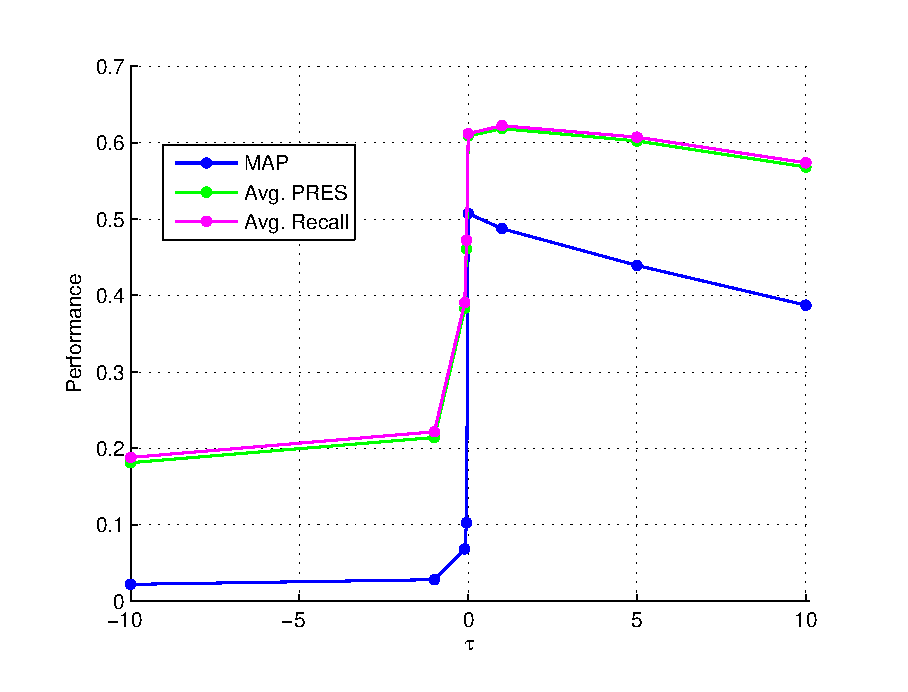
\epsfig{file=figs/extended-optquery-tau.eps, height=2in, width=3.1in}
%\caption{A sample black and white graphic (.eps format).}
%\end{figure}

\begin{figure*}[htpb]
\begin{center}
\noindent\begin{minipage}[b]{0.3\linewidth}
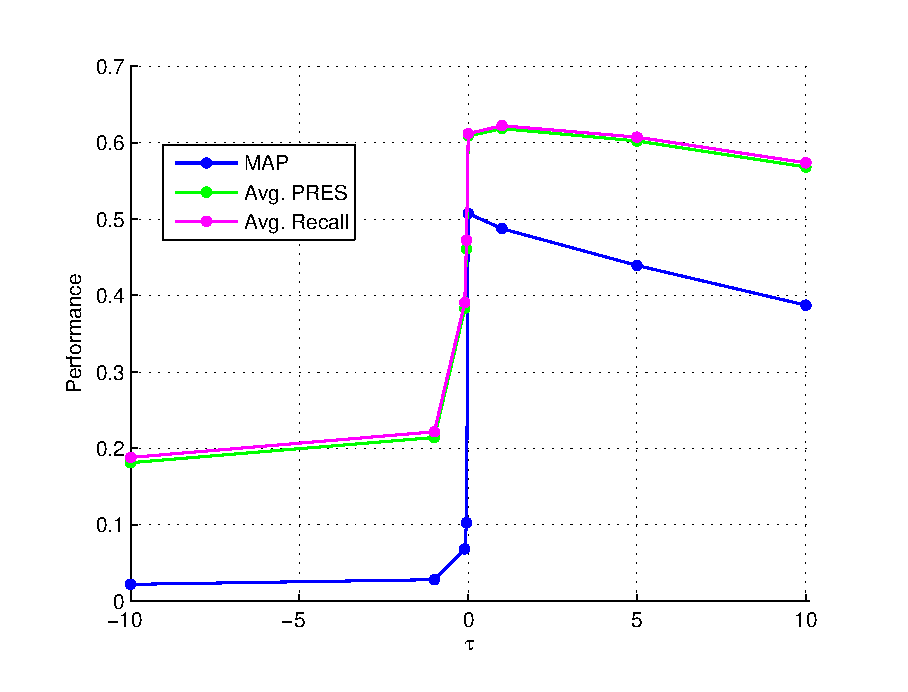
\includegraphics[width=\linewidth]{figs/extended-optquery-tau.eps}
\end{minipage}%
\hfill
%\hspace{7mm}
\begin{minipage}[b]{0.3\linewidth}
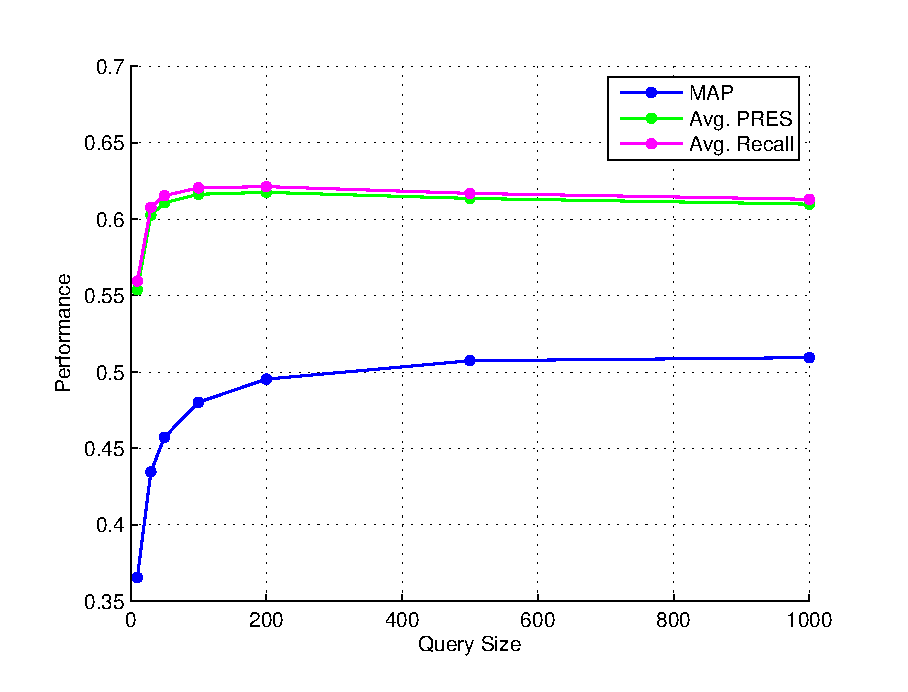
\includegraphics[width=\linewidth]{figs/opt-query-qsize.eps}
\end{minipage}
%\vspace{-3mm}\\
%(a) \hspace{30mm}(b)\\
\hfill
%\hspace{7mm}
\begin{minipage}[b]{0.3\linewidth}
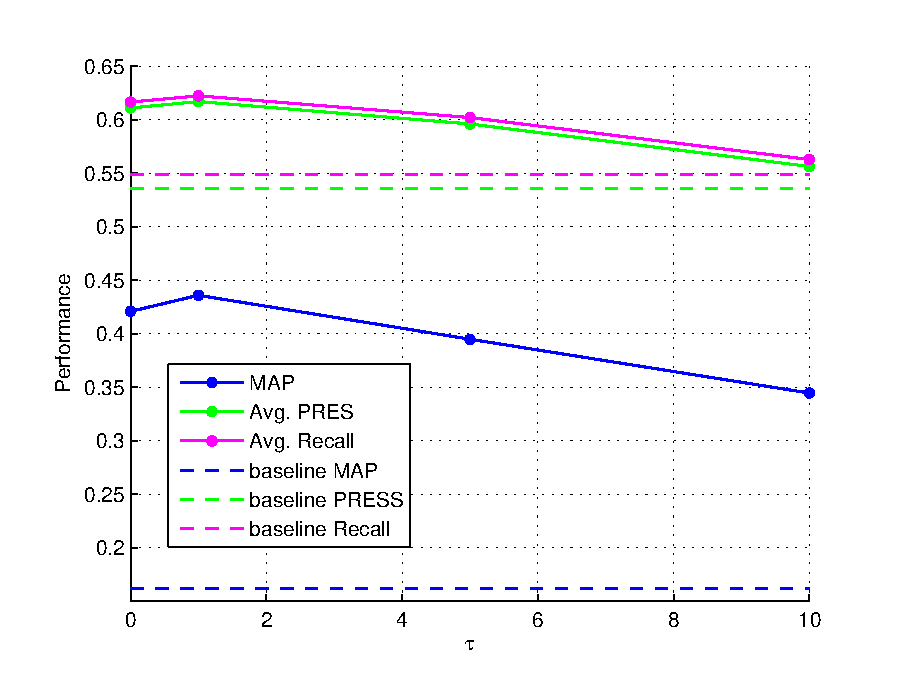
\includegraphics[width=\linewidth]{figs/opt-patentquery-tau.eps}
\end{minipage}
\vspace{-0.5mm}\\
 \hspace{2mm}(a) \hspace{55mm}(b) \hspace{58mm} (c)
\caption{\footnotesize
How score threshold($\tau$) and query size controls the performance.
(a) Performance versus the score threshold. (b) Performance versus the query size. (c) System performance when we reduced the query by RF: $ query = Q\cap (useful \; terms) $, where $ Q $ is the patent query and $ useful\; terms = \{t| score_{RF}(t)>\tau\} $.}
\vspace{-4mm}
\end{center}
\label{fig:control}
\end{figure*}

%\begin{figure}[htpb]
%\begin{center}
%\noindent\begin{minipage}[b]{0.5\linewidth}
%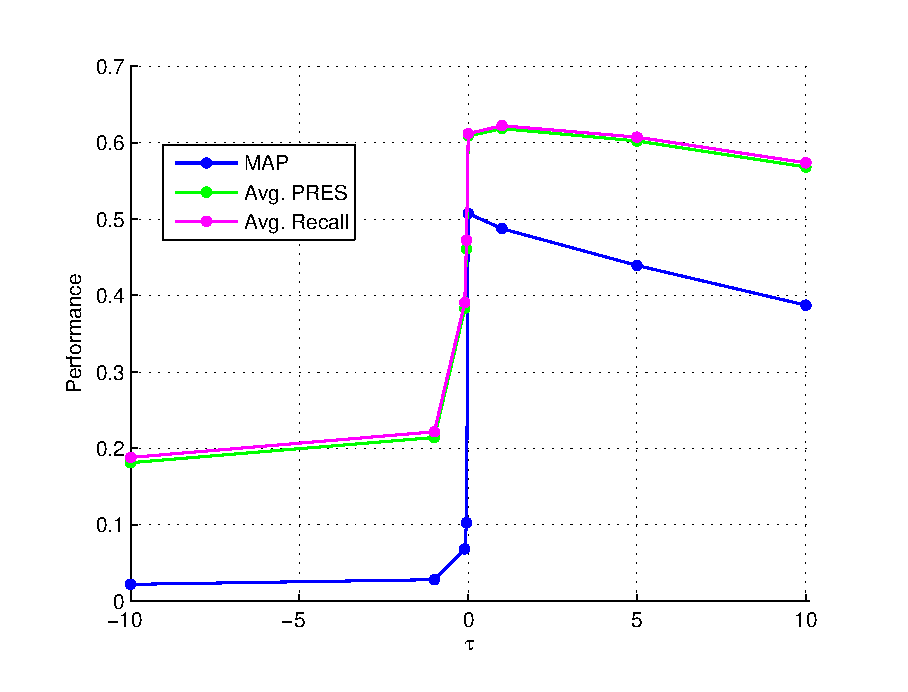
\includegraphics[width=\linewidth]{figs/extended-optquery-tau.eps}
%\end{minipage}%
%\hfill
%%\hspace{7mm}
%\begin{minipage}[b]{0.5\linewidth}
%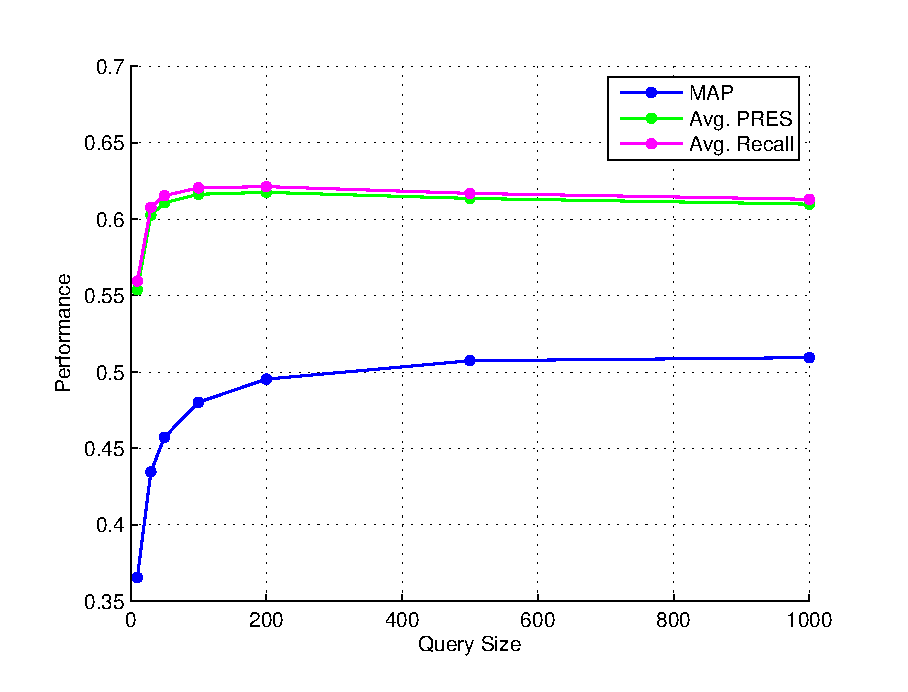
\includegraphics[width=\linewidth]{figs/opt-query-qsize.eps}
%\end{minipage}
%\vspace{-3mm}\\
%(a) \hspace{30mm}(b)\\
%%\hfill
%%\hspace{7mm}
%\begin{minipage}[b]{0.5\linewidth}
%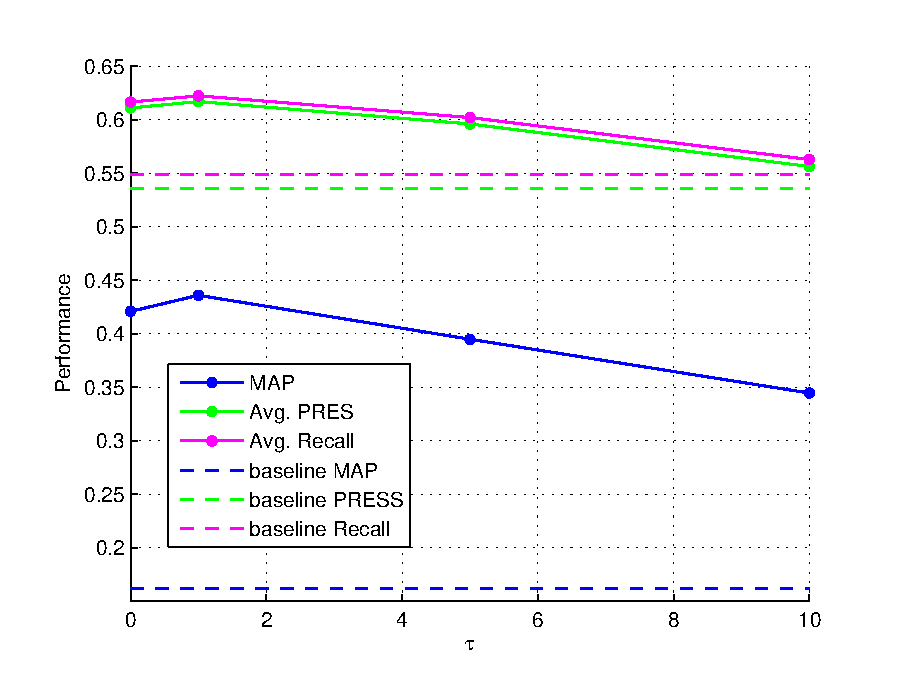
\includegraphics[width=\linewidth]{figs/opt-patentquery-tau.eps}
%\end{minipage}
%\vspace{-3mm}\\
%(c)
%\caption{\footnotesize
%How score threshold($\tau$) and query size controls the performance.
%(a) Performance versus the score threshold. (b) Performance versus the query size. (c) System performance when we reduced the query by RF: $ query = Q\cap (useful \; terms) $, where $ Q $ is the patent query and $ useful\; terms = \{t| score_{RF}(t)>\tau\} $.}
%\label{fig:mom2}
%\vspace{-4mm}
%\end{center}
%\label{fig:control}
%\end{figure}

\subsubsection{Query Reduction by Relevance Feedback}
Our experiments led us to another hypothesis that a patent query contains sufficient words matched with the relevant patents and the {\em noisy words} are the main cause of the low effectiveness. Therefore, we use RF {\em useful terms} to reduce the patent query terms by selecting terms such that: $ t \in \{ Q\cap (useful \; terms)\} $. Fig. (1-c) explicitly shows that a patent query contains sufficient words to retrieve relevant patents at top of the list. We only need to keep the {\em useful terms} and prune out the {\em noisy words}.
%\begin{figure}[htpb]
%   \centering
%   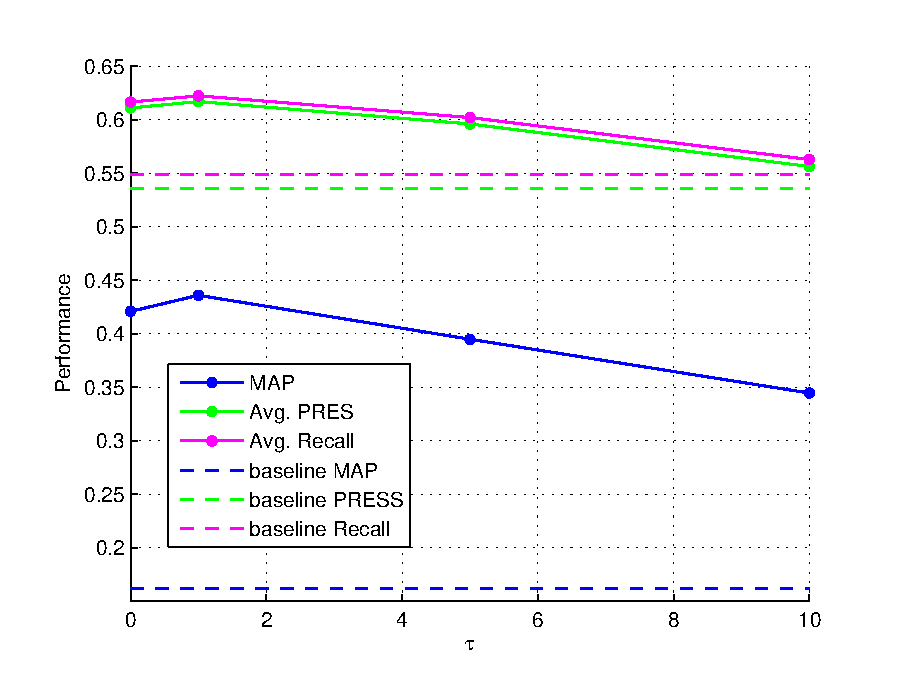
\includegraphics[width=0.3\textwidth,height=35mm]{figs/opt-patentquery-tau.eps}
%   \caption{Optimal patent query performance vs. score threshold of useful terms to select patent query terms. $ query = Q\cap (useful \; terms) $, where $ Q $ is the patent query and $ useful\; terms = \{t| score_{RF}(t)>\tau\} $..}   
%   \label{fig:optpatentquery} 
%\end{figure}

\subsection{What did not Work}
We achieved considerable improvement in performance using relevance feedback, however, it will cost to have a relevance feedback from our users who are professional patent examiners and recognizing a relevant patent is too demanding and time-taking. So, we tried other ways to refine the best query out of the patent query without an extended interaction. 
\subsubsection{Identify the Noisy Words}
First, we attempted to identify the noisy words. We hypothesized that the noisy words are frequent in top-100 retrieved documents. So, we calculate the average term frequency of each term as follows:
\begin{equation}
score_{DF}(t)= \frac{1}{100}\sum_{t\in \lbrace Top-100\rbrace} TF(t)  
 \label{eq:dfscore}
\end{equation}
where TF(t) is term frequency of each term in top-100 retrieved patent document. Fig. \ref{fig:dfrf} shows a scatter plot of RF score and Document Frequency(DF) score of words in top-100 retrieved documents.\vspace*{-2ex}
\begin{figure}[htpb]
   \centering
   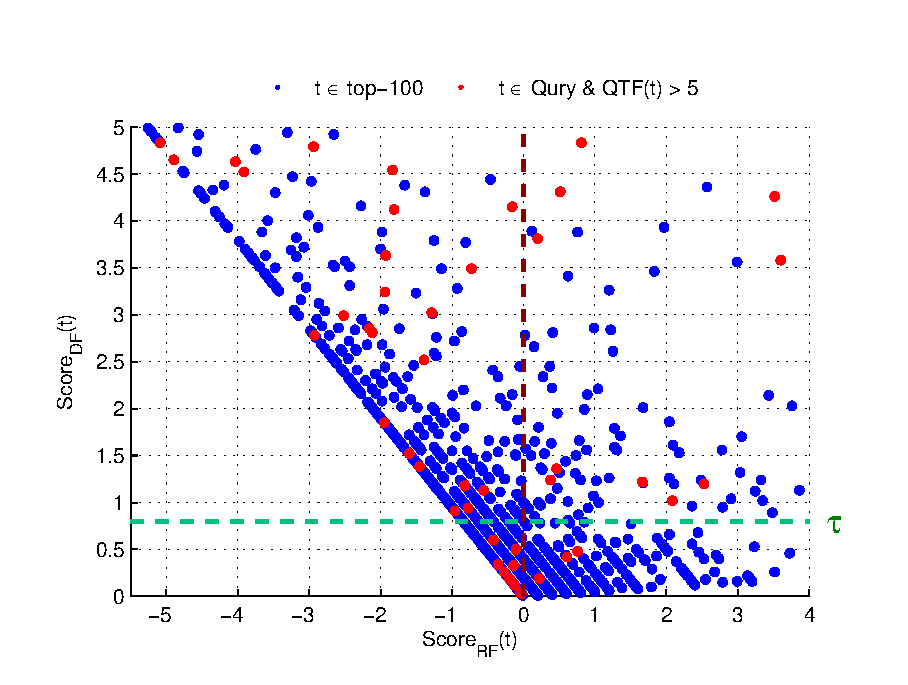
\includegraphics[width=0.30\textwidth,height=40mm]{figs/df-rf-tauline.eps}
   \caption{Anecdotal example: Scatter plot of $ score_{RF}(t) $ versus $ score_{DF}(t) $ for the words in top-100 retrieved documents. Each blue point is a vocabulary in top-100 retrieved document vocabulary set. Points highlighted in red are query words with term frequency higher than 5($ QTF(t)>5 $).}   
   \label{fig:dfrf} 
\end{figure}

\subsubsection{Pseudo Relevance Feedback(PRF)}
Pseudo relevance feedback or a blind feedback is precious since it is an automated process without user interaction which assumes that the top k ranked documents are relevant and the others are irrelevant. It has been found to improve performance in many applications, however we did not achieve the RF results by PRF. In fact, The results for PRF query formulation and query term selection using PRF were below the baseline. Fig. \ref{fig:anecdotal} explains the reason; it is an anecdotal example of a sample query with its abstract and a pair of PRF terms, with $ score_{PRF}(t)>10 $), and RF score of each term. It can be seen that terms with high PRF score are considered noise since their RF score is negative. Fig. \ref{fig:anecdotal} combined with Fig. 1-a can justify that terms from PRF are not useful at all because they contain sufficient noisy words to destruct the retrieval effectiveness. 
\begin{figure}[htpb]
\begin{framed}
\vspace*{-2ex}
  \centering
    %\lstinputlisting[frame=single, basicstyle=\scriptsize\ttfamily , linewidth=\columnwidth,breaklines=true]{code/anecdotale.tex}\vspace*{-2ex}
 \begin{lstlisting}[basicstyle=\tiny\ttfamily , linewidth=\columnwidth,breaklines=true] 
PAC-1612
Abstract: A wireless communication method for transmitting data from at least one master to one or more slaves positioned at various spatial locations and configured for generally simultaneous reception of the data. The method includes dividing the data into a number of portions, transmitting at least some of the portions using different transmission configurations for the different portions, having one or more of the slaves measure the quality of transmission associated with the group of different transmission configurations, and processing the quality measurements to determine new transmission configurations for use in transmitting the data.

PRF Terms: <@\textcolor{red}{commun:-69.43159}@>, <@\textcolor{red}{transmiss:-58.168427}@>, <@\textcolor{red}{wireless:-7.68421}@>, <@\textcolor{red}{telephon:-25.17895}@>, <@\textcolor{red}{recept:-37.810528}@>, <@\textcolor{red}{slave:-31.0421}@>, <@\textcolor{red}{deleg:-22.368422}@>, <@\textcolor{red}{turn:-18.536846}@>, <@\textcolor{red}{master:-35.778954}@>, <@\textcolor{red}{origin:-4.7473674}@>, <@\textcolor{blue}{schedul:12.852628}@>, <@\textcolor{red}{control:-14.842104}@>, <@\textcolor{blue}{frequenc:60.34737}@>, <@\textcolor{red}{station:-76.26316}@>, <@\textcolor{red}{electron:-8.442106}@>, <@\textcolor{red}{perform:-9.71579}@>, <@\textcolor{blue}{band:16.789476}@>, <@\textcolor{red}{termin:-40.04211}@>, <@\textcolor{blue}{indic:3.6210496}@>, <@\textcolor{red}{reason:-6.642107}@>, <@\textcolor{red}{apparatus:-6.2421055}@>, <@\textcolor{red}{determin:-8.97895}@>, <@\textcolor{red}{complet:-8.842103}@>, <@\textcolor{red}{prohibit:-3.8947372}@>, <@\textcolor{red}{state:-9.557897}@>, <@\textcolor{blue}{link:1.1157892}@>, <@\textcolor{blue}{hop:24.378946}@>, <@\textcolor{red}{lan:-8.3368435}@>, <@\textcolor{red}{assign:-9.68421}@>, <@\textcolor{blue}{f1:14.926317}@>, <@\textcolor{red}{short:-3.6000004}@>, <@\textcolor{blue}{pattern:17.58947}@>, <@\textcolor{blue}{paramet:1.5473672}@>, <@\textcolor{red}{serv:-4.5684214}@>, <@\textcolor{blue}{permit:0.62105286}@>
 \end{lstlisting} 
 \vspace*{-2ex}
\end{framed}
 \vspace*{-2ex}
  \caption{Anecdotal example: it shows the abstract and $ PRF term: \; score_{RF}(PRF term) $ pair of a sample query. Useful terms are highlighted in blue and the noisy ones in red.}
  \label{fig:anecdotal}  
\end{figure}
\vspace*{-2ex}
\subsection{Improvement by Minimum User Effort}
We could not improve the effectiveness without accessing the relevance feedback. In this experiment, we select query terms using only the first relevant patent document based on the hypothesis that a patent examiner can recognize the first relevant patent with minimum effort at top-5. Table \ref{tab:firstrel} shows that we can double the 'MAP' by using only the first-ranked relevant document.
\begin{table}[htpb]
  \begin{center}
   \caption{System performance when only the first relevant patent used for query reduction. $\tau$ is RF score threshold, and $k$ indicates the number of first relevant retrieved documents.}
  \input table/partialRFtermselect.tex   
  \label{tab:firstrel}
  \end{center}  
\end{table}

\begin{figure}[htpb]
   \centering
   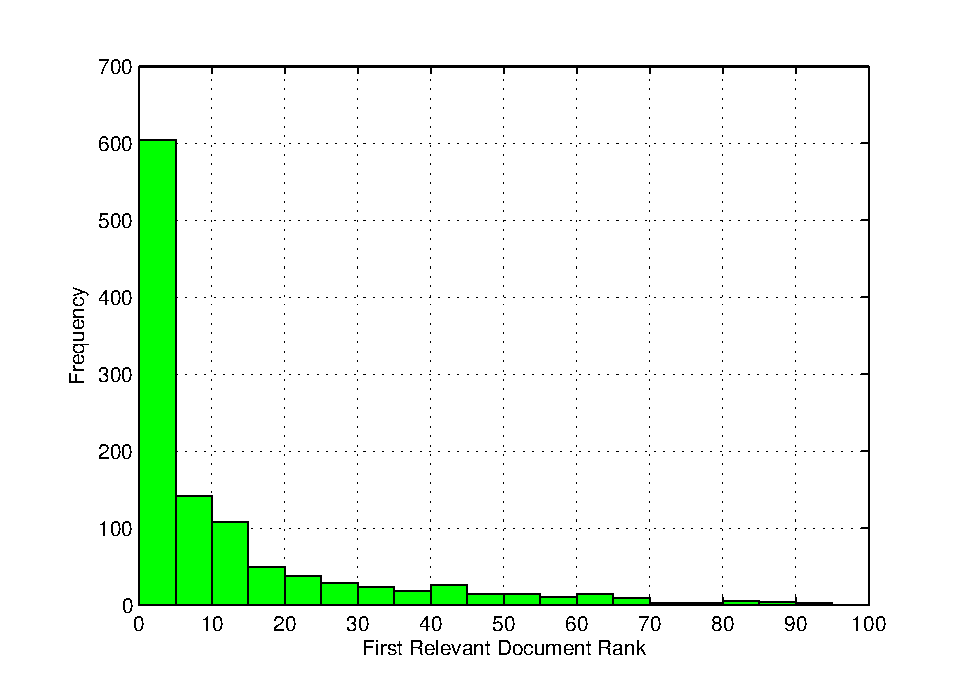
\includegraphics[width=0.25\textwidth,height=32mm]{figs/FirstTPRank.eps}
   \caption{The distribution of the first relevant document rank over test queries which have TPs}   
   \label{fig:FirstTPRankHisto} 
\end{figure}
\section{Related Work}

\section{Conclusions}

%\end{document}  % This is where a 'short' article might terminate

%ACKNOWLEDGMENTS are optional
\section{Acknowledgments}
NICTA is funded by the Australian Government as represented
by the Department of Broadband, Communications and the Digi-
tal Economy and the Australian Research Council through the ICT
Centre of Excellence program.


%
% The following two commands are all you need in the
% initial runs of your .tex file to
% produce the bibliography for the citations in your paper.
\bibliographystyle{abbrv}
\bibliography{sigproc}  % sigproc.bib is the name of the Bibliography in this case
% You must have a proper ".bib" file
%  and remember to run:
% latex bibtex latex latex
% to resolve all references
%
% ACM needs 'a single self-contained file'!
%
%APPENDICES are optional
%\balancecolumns
%\appendix
%%Appendix A
%\section{Headings in Appendices}
%The rules about hierarchical headings discussed above for
%the body of the article are different in the appendices.
%In the \textbf{appendix} environment, the command
%\textbf{section} is used to
%indicate the start of each Appendix, with alphabetic order
%designation (i.e. the first is A, the second B, etc.) and
%a title (if you include one).  So, if you need
%hierarchical structure
%\textit{within} an Appendix, start with \textbf{subsection} as the
%highest level. Here is an outline of the body of this
%document in Appendix-appropriate form:
%\subsection{Introduction}
%\subsection{The Body of the Paper}
%\subsubsection{Type Changes and  Special Characters}
%\subsubsection{Math Equations}
%\paragraph{Inline (In-text) Equations}
%\paragraph{Display Equations}
%\subsubsection{Citations}
%\subsubsection{Tables}
%\subsubsection{Figures}
%\subsubsection{Theorem-like Constructs}
%\subsubsection*{A Caveat for the \TeX\ Expert}
%\subsection{Conclusions}
%\subsection{Acknowledgments}
%\subsection{Additional Authors}
%This section is inserted by \LaTeX; you do not insert it.
%You just add the names and information in the
%\texttt{{\char'134}additionalauthors} command at the start
%of the document.
%\subsection{References}
%Generated by bibtex from your ~.bib file.  Run latex,
%then bibtex, then latex twice (to resolve references)
%to create the ~.bbl file.  Insert that ~.bbl file into
%the .tex source file and comment out
%the command \texttt{{\char'134}thebibliography}.
%% This next section command marks the start of
%% Appendix B, and does not continue the present hierarchy
%\section{More Help for the Hardy}
%The sig-alternate.cls file itself is chock-full of succinct
%and helpful comments.  If you consider yourself a moderately
%experienced to expert user of \LaTeX, you may find reading
%it useful but please remember not to change it.
%\balancecolumns % GM June 2007
% That's all folks!



\end{document}
